\documentclass[12pt,a4paper]{article}

% Packages
\usepackage{geometry}
\geometry{margin=1in}
\usepackage{fancyhdr}
\usepackage{titlesec}
\usepackage{listings}
\usepackage{xcolor}
\usepackage{graphicx} 

% Header & Footer
\pagestyle{fancy}
\fancyhf{}
\rhead{OOP Java - Assignment 4}
\lhead{Kamithkar Vinod}
\cfoot{\thepage}

% Title formatting
\titleformat{\section}{\large\bfseries}{Problem \thesection:}{0.5em}{}
\titleformat{\subsection}[runin]{\bfseries}{Code:}{0.5em}{}[---]
\titleformat{\subsubsection}[runin]{\bfseries}{Output:}{0.5em}{}[---]

% Code style
\lstset{
    language=Java,
    basicstyle=\ttfamily\small,
    keywordstyle=\color{blue}\bfseries,
    commentstyle=\color{gray}\itshape,
    stringstyle=\color{red},
    showstringspaces=false,
    numbers=left,
    numberstyle=\tiny\color{gray},
    frame=single,
    breaklines=true
}

% Document Start
\begin{document}

% Title Page
\begin{center}
    \LARGE \textbf{Assignment - 4} \\[0.5cm]
    \Large \textbf{Object-Oriented Programming in Java} \\[1cm]

    \begin{tabular}{rl}
        \textbf{Name:} & Kamithkar Vinod \\
        \textbf{Course:} & PG DAC AUGUST 2025 \\
        \textbf{Form No:} & 250500480 \\
        \textbf{Date:} & 14-09-2025 \\
    \end{tabular}
\end{center}

\vspace{1cm}
\hrule
\vspace{0.5cm}

% Problems

\section{Print Numbers 10 to 110}
\textbf{Task:} Write a program to print numbers 10 to 110.

\subsection{}
\begin{lstlisting}
class _1PrintNumbers {
    public static void main(String[] args) {
        for (int i = 10; i <= 110; i++) {
            System.out.print(i + " ");
        }
    }
}
\end{lstlisting}

\subsubsection{}
\begin{center}
    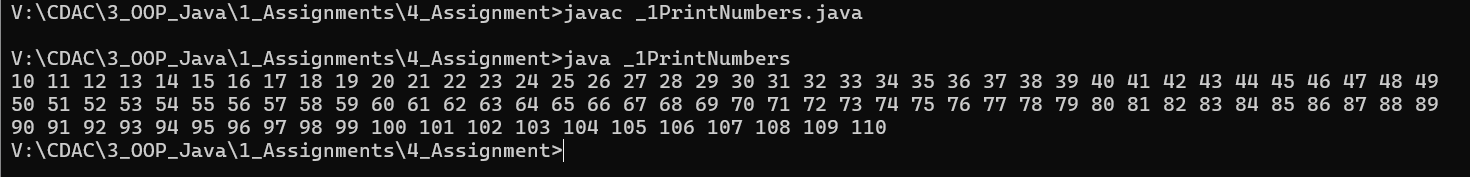
\includegraphics[width=0.8\textwidth]{Assignment - 4/4/1/1_print_numbers.png}
\end{center}

\section{Sum of All Numbers from 1 to 100}
\textbf{Task:} Write a program to calculate the sum of all numbers from 1 to 100.

\subsection{}
\begin{lstlisting}
class _2SumOfNumbers {
    public static void main(String[] args) {
        int sum = 0;
        for (int i=1; i<=100; i++) {
            sum += i;
        }
        System.out.println("Sum of No's 1 to 100: " + sum);
    }
}
\end{lstlisting}

\subsubsection{}
\begin{center}
    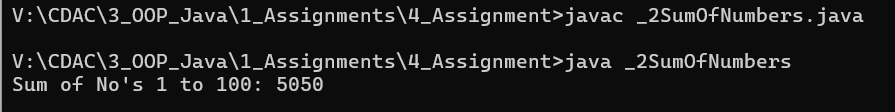
\includegraphics[width=0.8\textwidth]{Assignment - 4/4/1/2_sum_numbers.png}
\end{center}

\section{Multiplication Table of a Given Number}
\textbf{Task:} Write a program to print the multiplication table of a given number.

\subsection{}
\begin{lstlisting}
import java.util.Scanner;
class _3MultiplicationTable {
    public static void main(String[] args) {
        Scanner scanner = new Scanner(System.in);
        System.out.println("Enter the Number to do MultiplicationTable: ");
        int n = scanner.nextInt();
    
        for (int i=1; i<=10; i++) {
            System.out.println(n +" * "+ i + " = " + n*i);
        }
    }
}
\end{lstlisting}

\subsubsection{}
\begin{center}
    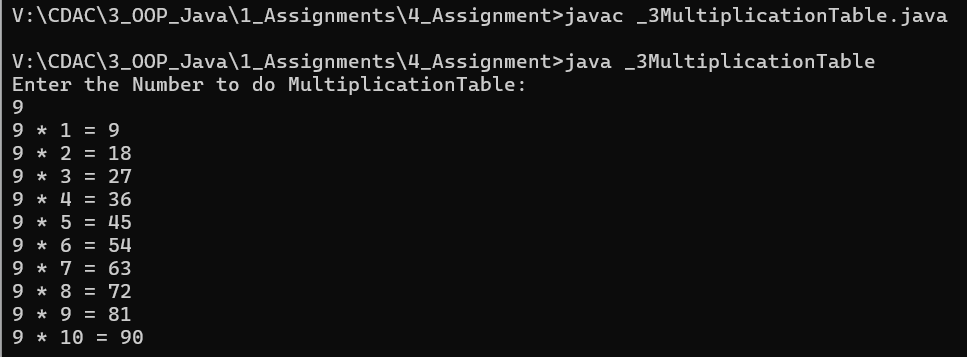
\includegraphics[width=0.8\textwidth]{Assignment - 4/4/1/3_multiplication_table.png}
\end{center}

\section{Factorial Given Number}
\textbf{Task:} Write a program to find the factorial of a given number.

\subsection{}
\begin{lstlisting}
import java.util.Scanner;
class _4Factorial {
    public static void main(String[] args) {
        Scanner scanner = new Scanner(System.in);
        System.out.print("Enter a Number to find factorial: ");
        int f = scanner.nextInt();
        int total = 1;
        for(int i=0; i<f; i++) {
            total *= (f-i);
        }
        System.out.println("The factorial of "+f+" is "+total);
    }
}
\end{lstlisting}

\subsubsection{}
\begin{center}
    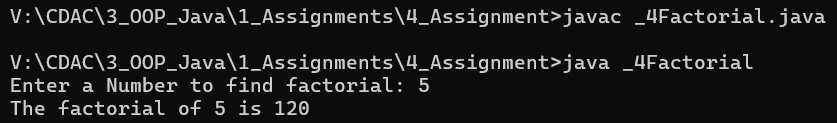
\includegraphics[width=0.8\textwidth]{Assignment - 4/4/1/4_factorial.png}
\end{center}

\section{Check Prime Number or Not}
\textbf{Task:} Write a program to check if a given number is prime.

\subsection{}
\begin{lstlisting}
class _5Prime {
    public static void main(String[] args) {
        // generate random number 1 to 1000
        int n = 1 + (int) (Math.random() * 1000);
        int count = 0, i;
    
        for(i=1; i<=n/2; i++) {
            if (n%i == 0){
                count++;
                if (count > 1)
                    break;
            }
        }
        System.out.println("No of iterations = " + (i-1));
        if (count == 1)
            System.out.println(n + " is a Prime Number");
        else
            System.out.println(n + " is not a Prime Number");
    }
}
\end{lstlisting}

\subsubsection{}
\begin{center}
    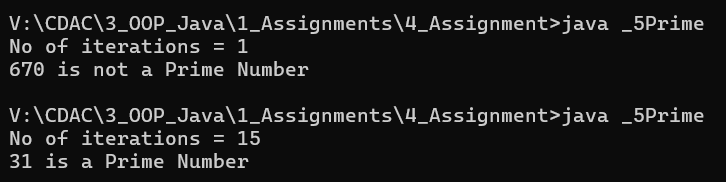
\includegraphics[width=0.8\textwidth]{Assignment - 4/4/1/5_prime_number.png}
\end{center}

\section{Fibonacci Series}
\textbf{Task:} Write a program to print the Fibonacci series up to a given number of terms.

\subsection{}
\begin{lstlisting}
class _6Fibonacci {
    public static void main(String[] args) {
        int n = 1 + (int) (Math.random()*10);
        int first = 0, second = 1;
    
        System.out.println("Fibonacci Series upto "+n+" terms: ");
    
        for(int i = 1; i<=n; i++){
            System.out.print(first + " ");
    
            int next = first + second;
            first = second;
            second = next;
        }
    }
}
\end{lstlisting}

\subsubsection{}
\begin{center}
    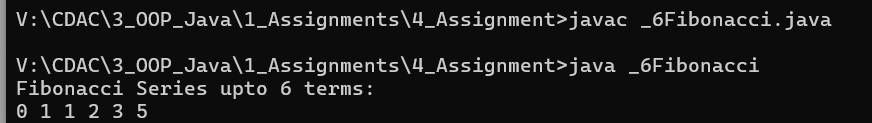
\includegraphics[width=0.8\textwidth]{Assignment - 4/4/1/6_fibo.png}
\end{center}

\section{Sum of digits of a Number}
\textbf{Task:} Write a program to calculate the sum of digits of a given number.

\subsection{}
\begin{lstlisting}
class _7SumOfDigits {
    public static void main(String[] args) {
        int num = 101 + (int) (Math.random() * 900);
        int sum = 0;
        int temp = num;
        
        while (temp != 0) {
            int digit = temp % 10;
            sum += digit;
            temp /= 10;
        }
        System.out.println("Sum of digits of "+num+" is :" + sum);
    }
}
\end{lstlisting}

\subsubsection{}
\begin{center}
    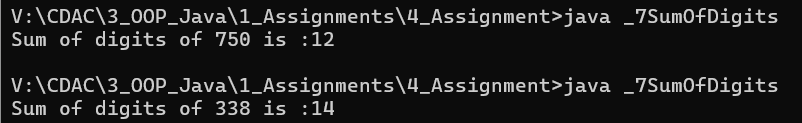
\includegraphics[width=0.8\textwidth]{Assignment - 4/4/1/7_sum_of_digits.png}
\end{center}

\section{Check Palindrome Number or Not}
\textbf{Task:} Write a program to check if a given number is a palindrome.

\subsection{}
\begin{lstlisting}
class _8Palindrome {
    public static void main(String[] args) {
    
        int num = 101 + (int) (Math.random() * 900);
        int original = num;
        int reversed = 0;
    
        while (num != 0) {
            int digit = num % 10;
            reversed = (reversed * 10) + digit;
            num /= 10;
        }
        if (original == reversed) 
            System.out.println(original + " is a Palindrome");
        else 
            System.out.println(original + " is not a Palindrome");
    }
}
\end{lstlisting}

\subsubsection{}
\begin{center}
    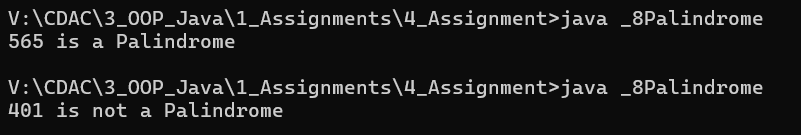
\includegraphics[width=0.8\textwidth]{Assignment - 4/4/1/8_palindrome.png}
\end{center}

\section{Odd Numbers 1 to 50}
\textbf{Task:} 9. Write a program to find the sum of all odd numbers between 1 and 50

\subsection{}
\begin{lstlisting}
class _9SumOfOdd {
    public static void main(String[] args) {
        int sum = 0;
        for(int i = 1; i<= 50; i++) {
            if (i % 2 != 0)
                sum += i;
        }
        System.out.println("Sum of Odd Numbers 1 to 50 is: "+sum);
    }
}
\end{lstlisting}

\subsubsection{}
\begin{center}
    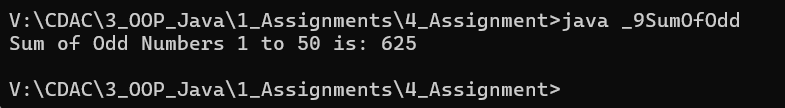
\includegraphics[width=0.8\textwidth]{Assignment - 4/4/1/9_sum_odd.png}
\end{center}

\section{Even Numbers 1 to 50}
\textbf{Task:} Write a program to find the sum of all even numbers between 1 and 50.

\subsection{}
\begin{lstlisting}
class _10SumOfEven {
    public static void main(String[] args) {
        int sum = 0;
        for(int i = 1; i<= 50; i++) {
            if (i % 2 == 0)
                sum += i;
        }
        System.out.println("Sum of Odd Numbers 1 to 50 is: "+sum);
    }
}
\end{lstlisting}

\subsubsection{}
\begin{center}
    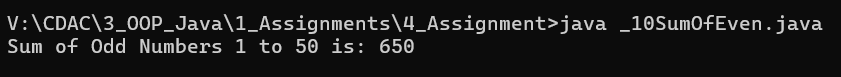
\includegraphics[width=0.8\textwidth]{Assignment - 4/4/1/10_sum_even.png}
\end{center}

% 11 to 20

\section{Check Armstrong Number}
\textbf{Task:} Write a program to check if a given number is Armstrong.

\subsection{}
\begin{lstlisting}
import java.util.Scanner;
class _11Armstrong {
    public static void main(String[] args) {
        Scanner scanner = new Scanner(System.in);
        System.out.print("Enter a Number: ");
        int num = scanner.nextInt();
    
        int sum = 0;
        int n = num;
    
        while (n != 0){
            int digit = n % 10;
            sum += Math.pow(digit, 3);
            n /= 10;
        }
        if (num == sum)
            System.out.println(num + " is an Armstrong Number");
        else 
            System.out.println(num + " is not an Armstrong Number");
    }
}
\end{lstlisting}

\subsubsection{}
\begin{center}
    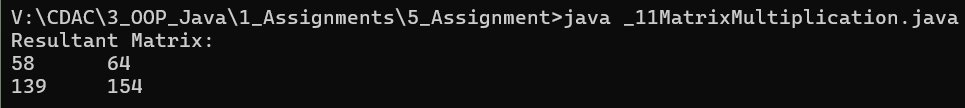
\includegraphics[width=0.8\textwidth]{Assignment - 4/4/2/11.png}
\end{center}

% 12

\section{Reverse Number}
\textbf{Task:} Write a program to reverse a given number.

\subsection{}
\begin{lstlisting}
class _12ReverseNumber {
    public static void main(String[] args) {
        int num = 101 + (int) (Math.random() * 900);
        int reverse = 0;
        int n = num;
        while(n != 0) {
            int digit = n % 10;
            reverse = (reverse * 10) + digit;
            n /= 10;
        }
        System.out.println("The reverse of "+num+" is: "+reverse);
    }
}
\end{lstlisting}

\subsubsection{}
\begin{center}
    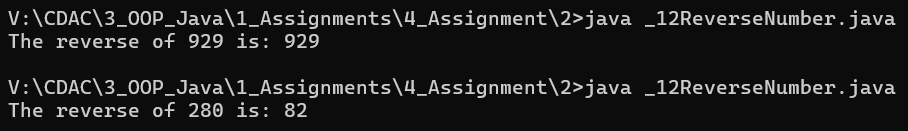
\includegraphics[width=0.8\textwidth]{Assignment - 4/4/2/12.png}
\end{center}

% 13

\section{Calculate Power of the loop}
\textbf{Task:} Write a program to calculate the power of a number using a loop.

\subsection{}
\begin{lstlisting}
import java.util.Scanner;
class _13PowerCalc {
    public static void main(String[] args) {
        Scanner scanner = new Scanner(System.in);
        System.out.print("Enter a Base Number: ");
        int base = scanner.nextInt();
        System.out.print("Enter a exponent: ");
        int exp = scanner.nextInt();
    
        long result = 1;
    
        for(int i=0; i<exp; i++){
            result *= base;
        }
        System.out.println(base+" to the power of "+exp+" = "+result);
    }
}
\end{lstlisting}

\subsubsection{}
\begin{center}
    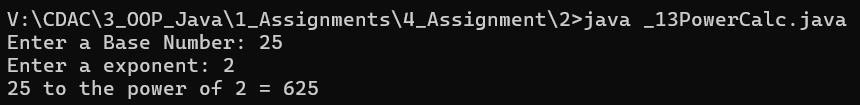
\includegraphics[width=0.8\textwidth]{Assignment - 4/4/2/13.png}
\end{center}

% 14

\section{GCD of Two Numbers}
\textbf{Task:} Write a program to find the greatest common divisor (GCD) of two numbers.

\subsection{}
\begin{lstlisting}
import java.util.Scanner;
class _14GCD {
    static int gcd(int a, int b) {
        while (b != 0) {
            int temp = b;
            b = a % b;
            a = temp;
        }
        return a;
    }
    public static void main(String[] args) {
        Scanner scanner = new Scanner(System.in);
        System.out.print("Enter First Number: ");
        int num1 = scanner.nextInt();
        System.out.print("Enter Second Number: ");
        int num2 = scanner.nextInt();
    
        // compute GCD
        int result = gcd(num1, num2);
    
        System.out.println("GCD of "+num1+" and "+num2+" is: "+result);
    }
}
\end{lstlisting}

\subsubsection{}
\begin{center}
    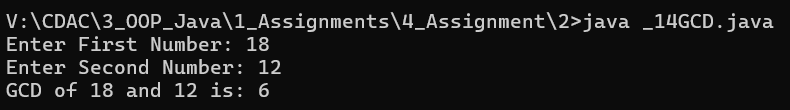
\includegraphics[width=0.8\textwidth]{Assignment - 4/4/2/14.png}
\end{center}

% 15

\section{String Palindrome}
\textbf{Task:} Write a program to check if a given string is a palindrome.

\subsection{}
\begin{lstlisting}
import java.util.Scanner;
class _15StringPalindrome {

    static boolean isPalindrome(String str, int left, int right) {
        if (left >= right) {
            return true;
        }
    
        if (str.charAt(left) != str.charAt(right)) {
            return false;
        }
        return isPalindrome(str, left+1, right-1);
    }
    
    public static void main(String[] args) {
        Scanner scanner = new Scanner(System.in);
        System.out.print("Enter a String: ");
        String str = scanner.nextLine();
        str = str.toLowerCase();
    
        if(isPalindrome(str, 0, str.length()-1)) {
            System.out.println(str + " is a String Palindrome");
        }
        else {
            System.out.println(str + " is not a String Palindrome");
        }
    }
}
\end{lstlisting}

\subsubsection{}
\begin{center}
    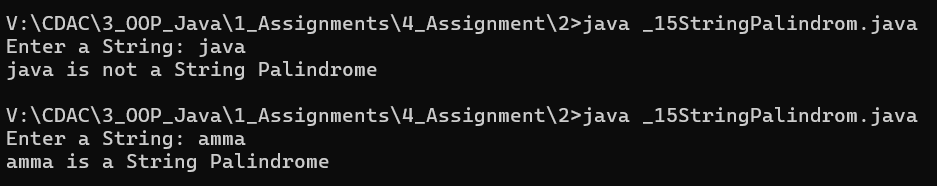
\includegraphics[width=0.8\textwidth]{Assignment - 4/4/2/15.png}
\end{center}

% 16

\section{ASCII lower case values}
\textbf{Task:} Write a program to print the ASCII values of all lowercase alphabets.

\subsection{}
\begin{lstlisting}
class _16LowerASCII {
    public static void main(String[] args) {
        System.out.println("Lower Case ASCII values: ");
        for (char ch = 'a'; ch<='z'; ch++) {
            System.out.print(ch + " -> " + (int) ch + " ");
        }
    }
}
\end{lstlisting}

\subsubsection{}
\begin{center}
    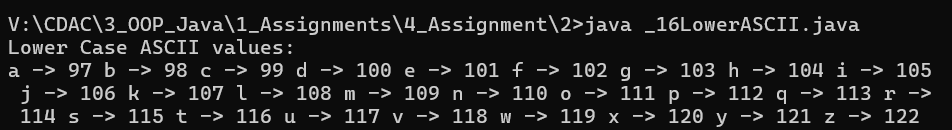
\includegraphics[width=0.8\textwidth]{Assignment - 4/4/2/16.png}
\end{center}

% 17

\section{Average of List of Numbers}
\textbf{Task:} 17. Write a program to calculate the average of a list of numbers.

\subsection{}
\begin{lstlisting}
import java.util.Scanner;
class _17AverageCalculator {
    public static void main(String[] args) {
        Scanner scanner = new Scanner(System.in);
        System.out.print("Enter the count of numbers: ");
        int n = scanner.nextInt();
    
        double sum = 0;
    
        for(int i=1; i<=n; i++) {
            double num = scanner.nextDouble();
            sum += num;
        }
    
        double avg = sum/n;
    
        System.out.println("Average = "+avg);
    }
}
\end{lstlisting}

\subsubsection{}
\begin{center}
    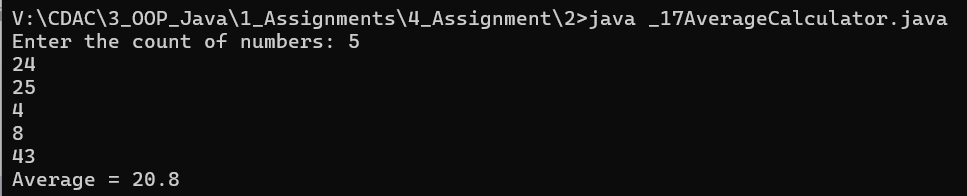
\includegraphics[width=0.8\textwidth]{Assignment - 4/4/2/17.png}
\end{center}

% 18

\section{Check Leap Year}
\textbf{Task:} Write a program to check if a given year is a leap year.

\subsection{}
\begin{lstlisting}
import java.util.Scanner;

class _18LeapYear {
    public static void main(String[] args) {
        Scanner scanner = new Scanner(System.in);
        System.out.print("Emter a year: ");
        int year = scanner.nextInt();
    
        if ((year%400==0) || ((year%4==0) && (year%100!=0)))
            System.out.println(year + " is a Leap Year");
        else
            System.out.println(year + " is not a Leap Year");
    }
}
\end{lstlisting}

\subsubsection{}
\begin{center}
    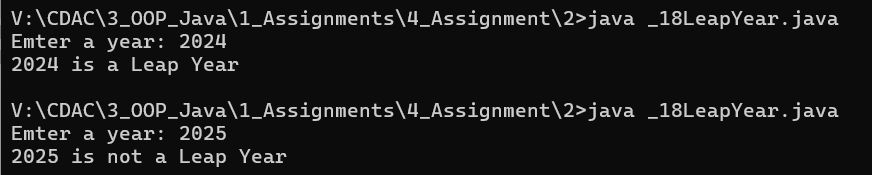
\includegraphics[width=0.8\textwidth]{Assignment - 4/4/2/18.png}
\end{center}

% 19

\section{10 Natural Numbers in reverse order}
\textbf{Task:} Write a program to print the first 10 natural numbers in reverse order.

\subsection{}
\begin{lstlisting}
class _19LastNatural {
    public static void main(String[] args) {
        System.out.println("First 10 Natural Numbers in reversed order : ");
    
        for(int i=10; i>=1; i--) {
            System.out.print(i + " ");
        }
    }
}
\end{lstlisting}

\subsubsection{}
\begin{center}
    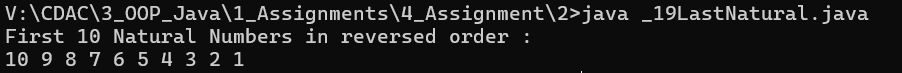
\includegraphics[width=0.8\textwidth]{Assignment - 4/4/2/19.png}
\end{center}

% 20

\section{Sum of First 50 Natural Numbers}
\textbf{Task:} Write a program to find the sum of the first 50 natural numbers.

\subsection{}
\begin{lstlisting}
class _20Sum50 {
    public static void main(String[] args) {
        int sum = 0;
    
        for (int i=1; i<=50; i++) {
            sum += i;
        }
        System.out.println("Sum of first 50 natural numbers: "+ sum);
    }
}
\end{lstlisting}

\subsubsection{}
\begin{center}
    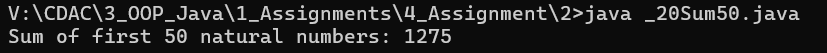
\includegraphics[width=0.8\textwidth]{Assignment - 4/4/2/20.png}
\end{center}

% 21 to 30

\section{Factorial Numbers 1 to 10}
\textbf{Task:} Write a program to print the factorial of numbers from 1 to 10.

\subsection{}
\begin{lstlisting}
class _21Factorial {
    public static void main(String[] args) {
        System.out.println("Factorial of Numbers from 1 to 10: ");
    
        long factorial = 1;
        for (int i=1; i<=10; i++) {
            factorial *= i;
            System.out.println(i + "! = " + factorial);
            }
        }
    }
\end{lstlisting}

\subsubsection{}
\begin{center}
    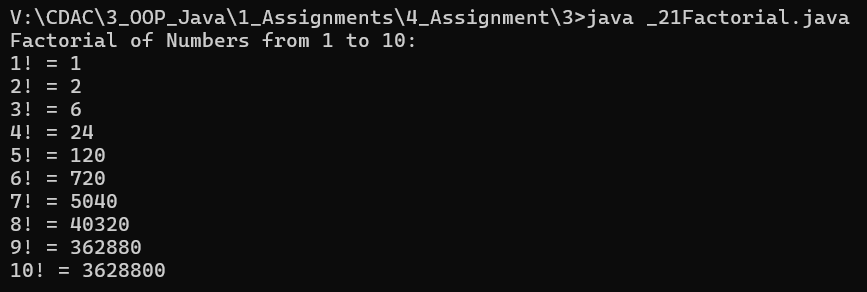
\includegraphics[width=0.8\textwidth]{Assignment - 4/4/3/21.png}
\end{center}

% 22

\section{String Palindrome using loop two pointer method}
\textbf{Task:} Write a program to check if a given string is a palindrome using a loop.

\subsection{}
\begin{lstlisting}
import java.util.Scanner;
class _15StringPalindromeLoop {
    public static void main(String[] args) {
        Scanner scanner = new Scanner(System.in);
        System.out.print("Enter a String: ");
        String str = scanner.nextLine();
        str = str.toLowerCase();
    
        int left = 0, right = str.length() - 1;
        boolean isPalindrome = true;
        // two pointer method
        while (left < right) {
            if (str.charAt(left) != str.charAt(right)){
                isPalindrome = false;
                break;
            }
            left++;
            right--;
        }
    
        if(isPalindrome) {
            System.out.println(str + " is a String Palindrome");
        }
        else {
            System.out.println(str + " is not a String Palindrome");
        }
    }
}
\end{lstlisting}

\subsubsection{}
\begin{center}
    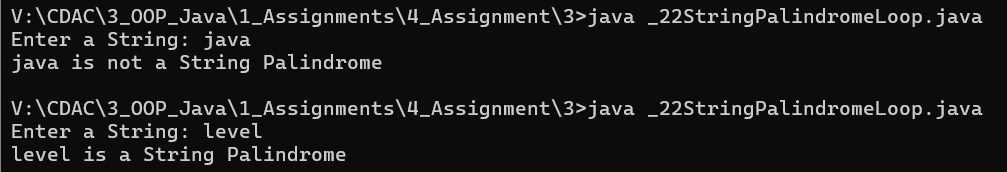
\includegraphics[width=0.8\textwidth]{Assignment - 4/4/3/22.png}
\end{center}

% 23

\section{Sum of Squares of Numbers 1 to 10}
\textbf{Task:} Write a program to calculate the sum of the squares of numbers from 1 to 10.

\subsection{}
\begin{lstlisting}
class _23SumSquares {
    public static void main(String[] args) {
    
        int sum = 0;
        for (int i=1; i<=10; i++) {
            sum += (int) Math.pow(i, 2);
        }
        System.out.println("Sum of first 10 square numbers: " + sum);
    }
}
\end{lstlisting}

\subsubsection{}
\begin{center}
    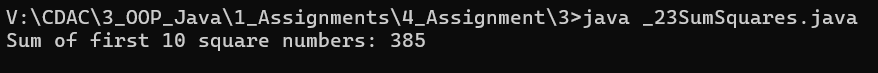
\includegraphics[width=0.8\textwidth]{Assignment - 4/4/3/23.png}
\end{center}

% 24

\section{Even Numbers 1 to 100}
\textbf{Task:} Write a program to print even numbers between 1 and 100.

\subsection{}
\begin{lstlisting}
class _24Even100 {
    public static void main(String[] args) {
        for (int i=2; i<=100; i++) {
            if (i%2==0)
                System.out.print(i + " ");
        }
    }
}
\end{lstlisting}

\subsubsection{}
\begin{center}
    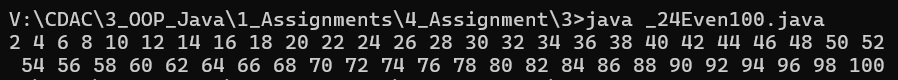
\includegraphics[width=0.8\textwidth]{Assignment - 4/4/3/24.png}
\end{center}

% 25

\section{Sum of Odd Numbers 1 to 50}
\textbf{Task:} Write a program to find the sum of all odd numbers between 1 and 50.

\subsection{}
\begin{lstlisting}
class _22SumOdd50 {
    public static void main(String[] args) {
        int sum = 0;
        for (int i=1; i<= 50; i++) {
            if (i%2!=0)
                sum += i;
        }
        System.out.print("Sum of 50 Odd Numbers: " + sum);
    }
}
\end{lstlisting}

\subsubsection{}
\begin{center}
    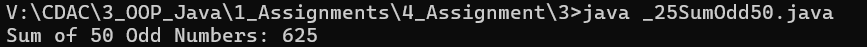
\includegraphics[width=0.8\textwidth]{Assignment - 4/4/3/25.png}
\end{center}

% 26

\section{Check Perfect Number}
A \textbf{perfect number} is a positive integer equal to the sum of its proper positive divisors (all divisors excluding the number itself). The first perfect number is $6$, as $1 + 2 + 3 = 6$. Other known perfect numbers include $28$, $496$, and $8128$. 

All known perfect numbers are even, and their form is described by the \textit{Euclid--Euler theorem}:
\[
2^{p-1} (2^p - 1)
\]
where $2^p - 1$ is a \textit{Mersenne prime}.

\textbf{Task:} Write a program to check if a given number is a perfect number.

\subsection{}
\begin{lstlisting}
import java.util.Scanner;

class _26PerfectNumber {
    public static void main(String[] args) {
        Scanner scanner = new Scanner(System.in);
        System.out.print("Enter a Number: ");
        int num = scanner.nextInt();
    
        // int sum = 0;
        
        // // find divisors and add
    
        // for (int i=1; i<=num/2; i++) {
        // 	if (num % i == 0) 
        // 		sum += i;
        // }
    
        // Efficient Java Implementation (O(√n))
        if (num <= 1){
            System.out.println(num + " is not a Perfect Number");
        }
    
        int sum = 1; // 1 is always a divisor
    
        // Check divisors up to sqrt(num)
    
        for (int i=2; i*i <= num; i++) {
            if (num % i == 0) {
                sum += i;
                if (i != num / i) {
                    sum += num / i; // add the pair divisor
                }
            }
        }
    
        // check perfect number
        if (num == sum && num > 0)
            System.out.println(num + " is a Perfect Number");
        else 
            System.out.println(num + " is not a Perfect Number");
    }
}
\end{lstlisting}

\subsubsection{}
\begin{center}
    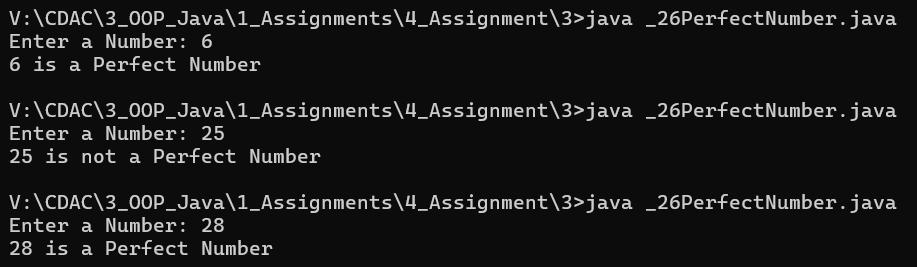
\includegraphics[width=0.8\textwidth]{Assignment - 4/4/3/26.png}
\end{center}

% 27

\section{Upper Case ASCII values}
\textbf{Task:} Write a program to print the ASCII values of all uppercase alphabets.

\subsection{}
\begin{lstlisting}
class _27UpperASCII {
    public static void main(String[] args) {
        for (char ch='A'; ch <= 'Z'; ch++) {
            System.out.print(ch + " -> " + (int) ch + " ");
        }
    }
}
\end{lstlisting}

\subsubsection{}
\begin{center}
    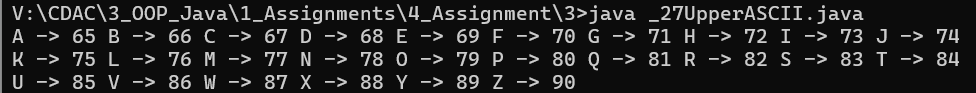
\includegraphics[width=0.8\textwidth]{Assignment - 4/4/3/27.png}
\end{center}

% 28

\section{Product of the digits of a number}
\textbf{Task:} Write a program to calculate the product of the digits of a given number.

\subsection{}
\begin{lstlisting}
import java.util.Scanner;
class _28ProductDigit {
    public static void main(String[] args) {
        Scanner scanner = new Scanner(System.in);
        System.out.print("Enter a Number: ");
        int num = scanner.nextInt();
    
        int n = num;
        int product = 1;
    
        while (n != 0) {
            int digit = n % 10;
            product *= digit;
            n /= 10;
        }
        System.out.println("Product of digits " + num + " is: "+ product);
    }
}
\end{lstlisting}

\subsubsection{}
\begin{center}
    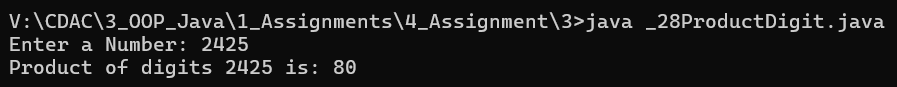
\includegraphics[width=0.8\textwidth]{Assignment - 4/4/3/28.png}
\end{center}

% 29

\section{Check Strong Number}
\textbf{Task:} Write a program to check if a given number is a strong number.

\subsection{}
\begin{lstlisting}
import java.util.Scanner;

class _29StrongNumber {
    
    // Method to calculate factorial
    static int factorial(int n) {
        int fact = 1;
        for (int i = 1; i <= n; i++) {
            fact *= i;
        }
        return fact;
    }
    
    public static void main(String[] args) {
        Scanner scanner = new Scanner(System.in);
    
        System.out.print("Enter a number: ");
        int num = scanner.nextInt();
    
        int temp = num;
        int sum = 0;
    
        // Calculate sum of factorial of digits
        while (temp != 0) {
            int digit = temp % 10;
            sum += factorial(digit);
            temp /= 10;
        }
    
        // Check if strong number
        if (sum == num) {
            System.out.println(num + " is a Strong Number.");
        } else {
            System.out.println(num + " is NOT a Strong Number.");
        }
    }
}
\end{lstlisting}

\subsubsection{}
\begin{center}
    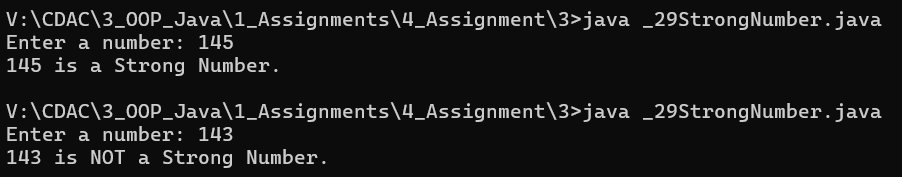
\includegraphics[width=0.8\textwidth]{Assignment - 4/4/3/29.png}
\end{center}

% 30

\section{Sum of Cubes 1 to 10}
\textbf{Task:} Write a program to calculate the sum of the cubes of numbers from 1 to 10.
You can also use the formula for the sum of the first $n$ cubes:

\[
1^3 + 2^3 + \cdots + n^3 = \left( \frac{n(n+1)}{2} \right)^2
\]

\subsection{}
\begin{lstlisting}
class _30SumCubes {
    public static void main(String[] args) {
        long total = 0;
        for (int i=1; i<=10; i++) {
            total += Math.pow(i, 3);
        }
        System.out.println("Sum of 1 to 10 cubes = " + total);
    }
}
\end{lstlisting}

\subsubsection{}
\begin{center}
    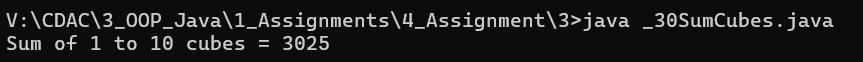
\includegraphics[width=0.8\textwidth]{Assignment - 4/4/3/30.png}
\end{center}

% 31 to 40

\section{Sum of Prime Numbers 1 to 100}
\textbf{Task:} Write a program to find the sum of all prime numbers between 1 and 100.

\subsection{}
\begin{lstlisting}
class _31PrimeNumbers {

    public static void main(String[] args) {
        System.out.println("Prime numbers from 1 to 100 are:");
    
        int sum = 0;
        for (int i = 2; i <= 100; i++) {
            boolean isPrime = true;
    
            // This is an optimized approach, as a number's factors repeat after its square root.
            for (int j = 2; j <= Math.sqrt(i); j++) {
                // If the number is divisible by any 'j', it's not prime.
                if (i % j == 0) {
                    isPrime = false;
                    break; 
                }
            }
            if (isPrime) {
                System.out.print(i + " ");
                sum += i;
            }
        }
        System.out.println("Sum of 1 to 100 primes = " + sum);
    }
}

\end{lstlisting}

\subsubsection{}
\begin{center}
    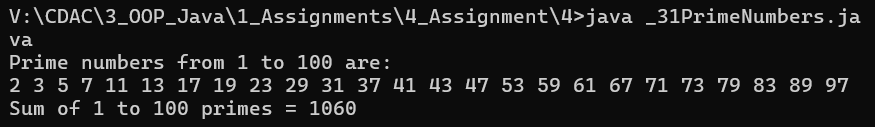
\includegraphics[width=0.8\textwidth]{Assignment - 4/4/4/31.png}
\end{center}

% 32

\section{Check Pangram}
\textbf{Task:} Write a program to check if a given string is a pangram.

\subsection{}
\begin{lstlisting}
import java.util.Scanner;
class _32Panagram {
    public static void main(String[] args) {
        Scanner scanner = new Scanner(System.in);
        System.out.println("Enter a String: ");
        String str = scanner.nextLine().toLowerCase();
        String alphabet = "abcdefghijklmnopqrstuvwxyz";
    
        int count = 0;
    
        for (int i = 0; i<26; i++) {
            if (str.indexOf(alphabet.charAt(i)) != -1) {
                count++;
            }
        }
    
        if (count == 26)
            System.out.println("Given String is a Panagram");
        else
            System.out.println("Not a Panagram");
    }
}
\end{lstlisting}

\subsubsection{}
\begin{center}
    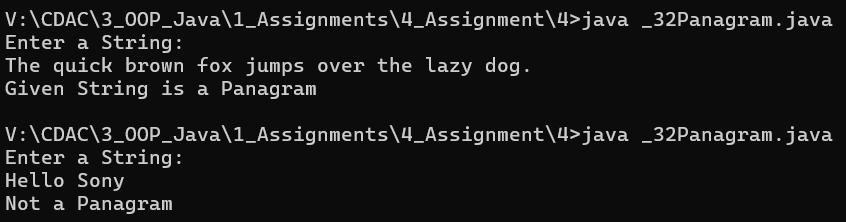
\includegraphics[width=0.8\textwidth]{Assignment - 4/4/4/32.png}
\end{center}

% 33

\section{Factorial Numbers 1 to 10}
\textbf{Task:} Write a program to find the factorial of numbers from 1 to 10.

\subsection{}
\begin{lstlisting}
class _21Factorial {
    public static void main(String[] args) {
        System.out.println("Factorial of Numbers from 1 to 10: ");
    
        long factorial = 1;
        for (int i=1; i<=10; i++) {
            factorial *= i;
            System.out.println(i + "! = " + factorial);
            }
        }
	}
\end{lstlisting}

\subsubsection{}
\begin{center}
    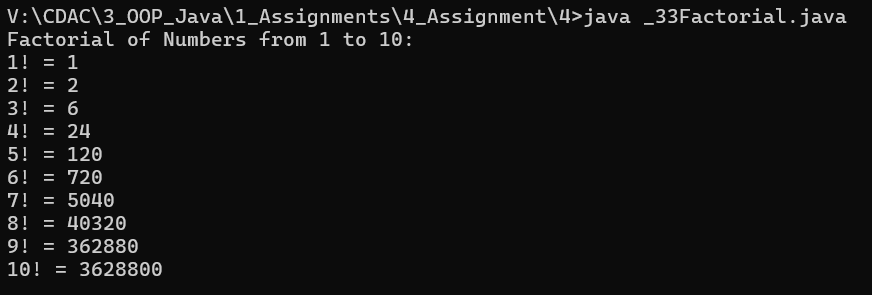
\includegraphics[width=0.8\textwidth]{Assignment - 4/4/4/33.png}
\end{center}

% 34

\section{Odd Numbers 1 to 100}
\textbf{Task:} Write a program to print odd numbers between 1 and 100.

\subsection{}
\begin{lstlisting}
class _34OddNumbers {
    public static void main(String[] args) {
        for(int i=1; i<=100; i++) {
            if (i%2 != 0) {
                System.out.print(i + " ");
            }
        }
    }
}
\end{lstlisting}

\subsubsection{}
\begin{center}
    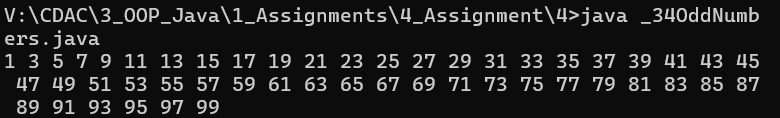
\includegraphics[width=0.8\textwidth]{Assignment - 4/4/4/34.png}
\end{center}

% 35

\section{Check Perfect Square}
\textbf{Task:} Write a program to check if a given number is a perfect square.

\subsection{}
\begin{lstlisting}
import java.util.Scanner;
class _35PerfectSquare {
    public static void main(String[] args) {
        Scanner scanner = new Scanner(System.in);
        System.out.print("Enter a Number: ");
        int num = scanner.nextInt();
        int i;
        // negative numbers are not perfect square
        // zero is a perfect square
        for (i=0; i*i <= num; i++) {
            if (i*i == num) {
                System.out.println(num + " is a Perfect Square");
                break;
            }
        }
        if (i*i > num) {
            System.out.println(num + " is not a Perfect Square");
        }
    }
}
\end{lstlisting}

\subsubsection{}
\begin{center}
    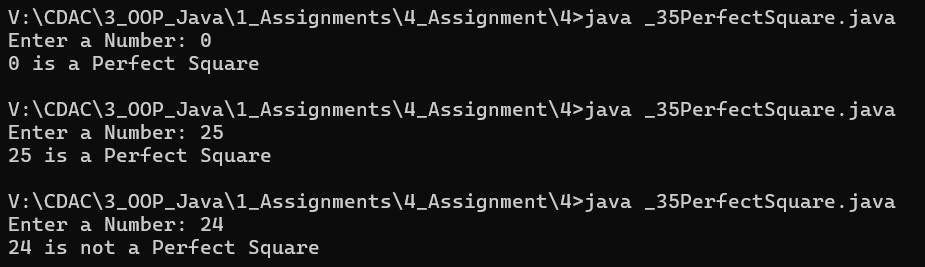
\includegraphics[width=0.8\textwidth]{Assignment - 4/4/4/35.png}
\end{center}

% 36

\section{Sum of the digits}
\textbf{Task:} Write a program to find the sum of the digits of a given number until the sum is a single digit.

\subsection{}
\begin{lstlisting}
import java.util.Scanner;

class _36SinglDigitRoot {
    public static void main(String[] args) {
        Scanner sc = new Scanner(System.in);
    
        System.out.print("Enter a number: ");
        int num = sc.nextInt();
    
        // Reduce until single digit
        int result = num;
        while (result >= 10) {
            result = sumOfDigits(result);
        }
    
        System.out.println("The single digit sum is: " + result);
    }
    
    public static int sumOfDigits(int n) {
        int sum = 0;
        while (n > 0) {
            sum += n % 10; // add last digit
            n /= 10;       // remove last digit
        }
        return sum;
    }
}
\end{lstlisting}

\subsubsection{}
\begin{center}
    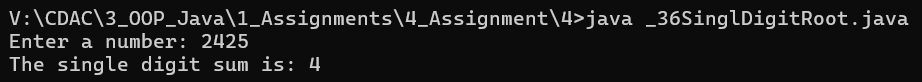
\includegraphics[width=0.8\textwidth]{Assignment - 4/4/4/36.png}
\end{center}

% 37

\section{Square Pattern}
\textbf{Task:} Square Pattern

\subsection{}
\begin{lstlisting}
class _37SquarePattern {
    public static void main(String[] args) {
        for (int i=1; i<=5; i++) {
            System.out.println();
            for (int j=1; j<=5; j++) {
                System.out.print(" * ");
            }
        }
    }
}
\end{lstlisting}

\subsubsection{}
\begin{center}
    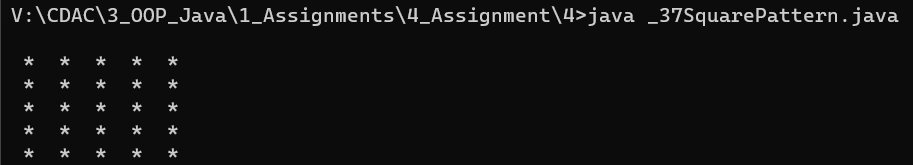
\includegraphics[width=0.8\textwidth]{Assignment - 4/4/4/37.png}
\end{center}

% 38

\section{Right Angled Triangle}
\textbf{Task:} Right Angled Triangle

\subsection{}
\begin{lstlisting}
class _38RightAngledTriangle {
    public static void main(String[] args) {
        for (int i=1; i<=5; i++) {
            System.out.println();
            for (int j=1; j<=i; j++) {
                System.out.print("* ");
            }
        }
    }
}
\end{lstlisting}

\subsubsection{}
\begin{center}
    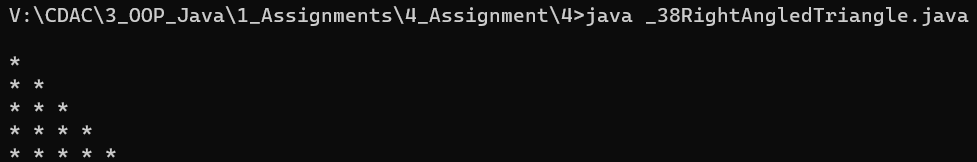
\includegraphics[width=0.8\textwidth]{Assignment - 4/4/4/38.png}
\end{center}

% 39

\section{Inverted Right Triangle}
\textbf{Task:} Inverted Right Triangle

\subsection{}
\begin{lstlisting}
class _39InvertedRightAngledTriangle {
    public static void main(String[] args) {
        for (int i=5; i>=1; i--) {
            System.out.println();
            for (int j=1; j<=i; j++) {
                System.out.print("* ");
            }
        }
    }
}
\end{lstlisting}

\subsubsection{}
\begin{center}
    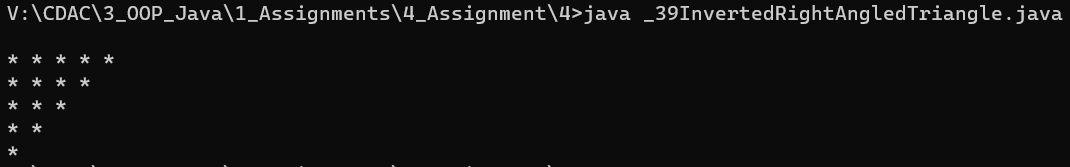
\includegraphics[width=0.8\textwidth]{Assignment - 4/4/4/39.png}
\end{center}

% 40

\section{Pyramid}
\textbf{Task:} Pyramid

\subsection{}
\begin{lstlisting}
class _40Pyramid {
    public static void main(String[] args) {
    
        int n = 5;
        for(int i=1; i<=n; i++) {
            for(int j=i; j<n; j++) System.out.print(" ");
            for(int j=1; j<=i; j++) System.out.print("* ");
            System.out.println();
        }
    }
}
\end{lstlisting}

\subsubsection{}
\begin{center}
    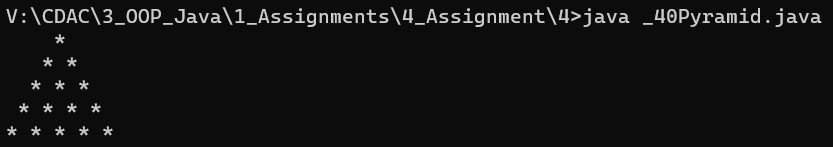
\includegraphics[width=0.8\textwidth]{Assignment - 4/4/4/40.png}
\end{center}

% 41

\section{Inverted Pyramid}
\textbf{Task:} Inverted Pyramid

\subsection{}
\begin{lstlisting}
class _41InvertedPyramid {
    public static void main(String[] args) {
    
        int n = 5;
        for(int i=n; i>=1; i--) {
            for(int j=i; j<n; j++) System.out.print(" ");
            for(int j=1; j<=i; j++) System.out.print("* ");
            System.out.println();
        }
    
    }
}
\end{lstlisting}

\subsubsection{}
\begin{center}
    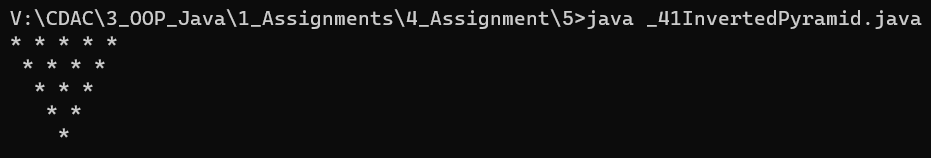
\includegraphics[width=0.8\textwidth]{Assignment - 4/4/5/41.png}
\end{center}

% 42

\section{Diamond}
\textbf{Task:} Diamond

\subsection{}
\begin{lstlisting}
class _42Diamond {
    public static void main(String[] args) {
    
        int n=3;
        // upper
        for(int i=1; i<=n; i++) {
            for(int j=i; j<n; j++) System.out.print(" ");
            for(int j=1; j<=i; j++) System.out.print("* ");
            System.out.println();
        }
        // lower
        for(int i=n-1; i>=1; i--) {
            for(int j=i; j<n; j++) System.out.print(" ");
            for(int j=1; j<=i; j++) System.out.print("* ");
            System.out.println();
        }
    }
}
\end{lstlisting}

\subsubsection{}
\begin{center}
    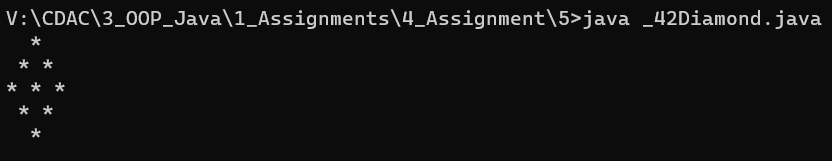
\includegraphics[width=0.8\textwidth]{Assignment - 4/4/5/42.png}
\end{center}

% 43

\section{Hallow Square}
\textbf{Task:} Hallow Square

\subsection{}
\begin{lstlisting}
class _43HollowSquare {
    public static void main(String[] args) {
        int n=5;
        for(int i=1; i<=n; i++) {
            for(int j=1; j<=n; j++) {
                if(i==1 || i==n || j==1 || j==n)
                    System.out.print("* ");
                else
                    System.out.print("  ");
                    }
            System.out.println();
        }
    }
}

\end{lstlisting}

\subsubsection{}
\begin{center}
    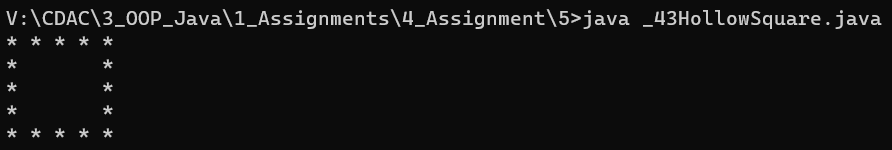
\includegraphics[width=0.8\textwidth]{Assignment - 4/4/5/43.png}
\end{center}

% 44

\section{Floyd's Triangle}
\textbf{Task:} Floyd's Triangle

\subsection{}
\begin{lstlisting}
class _44FloydTriangle {
    public static void main(String[] args) {
        int n=5, num=1;
        for (int i=1; i<=n; i++) {
            for (int j=1; j<=i; j++) {
                System.out.print(num++ + " ");
            }
            System.out.println();
        }
    }
}
\end{lstlisting}

\subsubsection{}
\begin{center}
    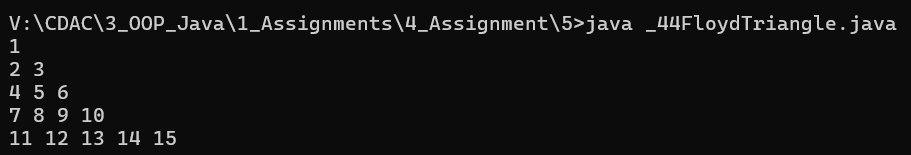
\includegraphics[width=0.8\textwidth]{Assignment - 4/4/5/44.png}
\end{center}

% 45

\section{Pascal Triangle}
\textbf{Task:} Pascal Triangle

\subsection{}
\begin{lstlisting}
class _45PascalTriangle {
    public static void main(String[] args) {
        int n = 4;
        for (int i=0; i<n; i++) {
            for (int j=0; j<n-i; j++) System.out.print("  ");
            int num = 1;
            for (int j=0; j<=i; j++) {
                System.out.print(num + "   ");
                num = num * (i-j)/(j+1);
            }
            System.out.println();
        }
    }
}
\end{lstlisting}

\subsubsection{}
\begin{center}
    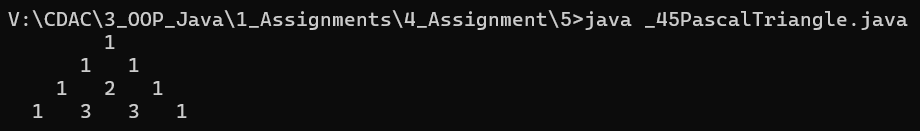
\includegraphics[width=0.8\textwidth]{Assignment - 4/4/5/45.png}
\end{center}

% 46

\section{Number Triangle}
\textbf{Task:} Number Triangle

\subsection{}
\begin{lstlisting}
class _46NumberTriangle {
    public static void main(String[] args) {
        for (int i=1; i<=4; i++) {
            for (int j=1; j<=i; j++) {
                System.out.print(j + " ");
            }
            System.out.println();
        }
    }
}
\end{lstlisting}

\subsubsection{}
\begin{center}
    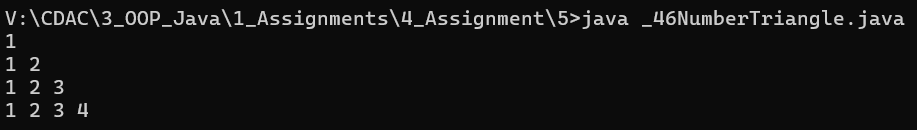
\includegraphics[width=0.8\textwidth]{Assignment - 4/4/5/46.png}
\end{center}

\end{document}
